%! Author = nadutkinfedor
%! Date = 09.01.2024

% Preamble
\documentclass[11pt]{article}
\usepackage[left=2cm, right=1cm, top=2cm, bottom=2cm, bindingoffset=0cm]{geometry}

% Packages
\usepackage[utf8]{inputenc}
\usepackage[russian]{babel}
\usepackage{amsmath}
\usepackage{hyperref}
\usepackage{graphicx}
\usepackage{misccorr}
\usepackage{listings}
\usepackage{xcolor}
\usepackage{titlesec}
\usepackage{minted}
\usepackage{color}
\usepackage{enumitem}
\usepackage{indentfirst}

%listing settings
\definecolor{dkgreen}{rgb}{0,0.6,0}
\definecolor{gray}{rgb}{0.5,0.5,0.5}
\definecolor{mauve}{rgb}{0.58,0,0.82}

\lstset{language=SQL,
    basicstyle={\small\ttfamily},
    belowskip=3mm,
    breakatwhitespace=true,
    breaklines=true,
    classoffset=0,
    columns=flexible,
    commentstyle=\color{dkgreen},
    framexleftmargin=0.25em,
    keywordstyle=\color{blue},
    numbers=none, %If you want line numbers, set `numbers=left`
    numberstyle=\tiny\color{gray},
    showstringspaces=false,
    stringstyle=\color{mauve},
    tabsize=3,
    xleftmargin =1em,
    backgroundcolor=\color{gray!10}
}

\lstset{ %
    backgroundcolor=\color{white},   % choose the background color
    basicstyle=\footnotesize,        % size of fonts used for the code
    breaklines=true,                 % automatic line breaking only at whitespace
    captionpos=b,                    % sets the caption-position to bottom
    commentstyle=\color{dkgreen},    % comment style
    escapeinside={\%*}{*},          % if you want to add LaTeX within your code
    keywordstyle=\color{blue},       % keyword style
    stringstyle=\color{mauve},     % string literal style
}

% Title
\title{DB internals. Вторая лекция}
\author{Надуткин Федор }
\date{December 2023}

\titleformat{\section}[block]{\Huge\bfseries\filcenter}{}{1em}{}
\titleformat{\subsection}[block]{\huge\bfseries\filcenter}{}{1em}{}
\titleformat{\subsubsection}[block]{\Large\bfseries\filcenter}{}{1em}{}

% Document
\begin{document}

    \maketitle

    \newpage

    \section*{Метаданные операторов}

    Не всегда ясно, как лучше проводить оптимизацию (например как лучше поменять порядок \texttt{Join}), поэтому на помощь приходят метаданные.
    Чем больше мы знаем о природе данных, возвращаемых оператором, тем больше полезных оптимизаций можно применить.

    \textbf{Метаданные} --- конкретные значения/структуры, которые мы можем извлечь из конкретного узла.

    \begin{lstlisting}[language=Java,label={lst:plan_node}]
        interface PlanNode {
            List<PlanNode> getInputs ( );
            T accept (PlanVisitor<T> visitor);
        }
    \end{lstlisting}

    \begin{lstlisting}[language=Java, label={lst:visitor}]
        interface PlanVisitor<T> {
            T visitScan (Scan node);
            T visitProject(Project node);
            T visitFilter (Filter node);
            T visitAggregate (Aggregate node);
            T visitJoin(Join node);
        }
    \end{lstlisting}

    \begin{itemize}
        \item Расчёт метаданных происходит рекурсивно.
        Перед тем как получить метаданные оператора, надо получить метаданные дочерних операторов.
        \item Зачастую метаданные могут повторяться, поэтому иногда их стоит кешировать.
    \end{itemize}

    \newpage

    \subsection*{Статистики}

    \textbf{Статистики} --- метаданные, которые приблизительно или точно описывают значения атрибутов.

    \begin{itemize}
        \item Row count --- сколько записей возвращает оператор.
        Важнейший фактор оценки стоймости операторов.
        \item Min/Max --- для оценки селективности предикатов.
        \item Null count --- для достаточно частого запроса \texttt{not null}
        \item NDV (number of distinct values) --- помогает оценить стоймость работы таких операторов как Aggregate или Join.
        Могут быть рассчитаны не только для отдельных атрибутов, но и для их комбинаций.
        \item Гистограммы --- распределение значений атрибутов.
    \end{itemize}

    \begin{figure}[h!]
        \centering
        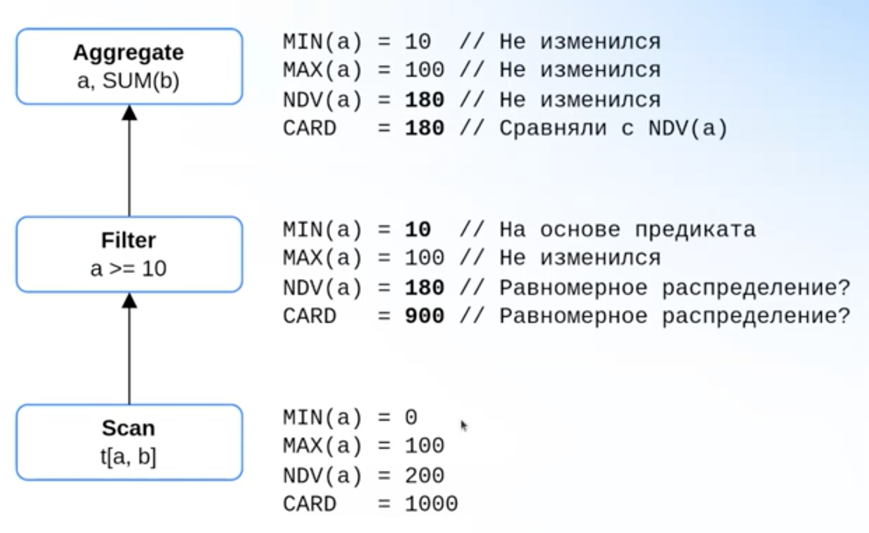
\includegraphics[width = \textwidth]{Pictures/Metadata/Рассчёт статистик}
        \caption{Пример расчёта статистики. (CARD - координальность оператора)}
        \label{fig:counting_statistics}
    \end{figure}

    \begin{enumerate}
        \item Для листьев плана статистики представляет движок.
        \item Для остальных операторов, статистики рассчитываются на основе статистик входов.
        \begin{itemize}
            \item Эвристики - наиболее распространённый подход, однако неточный.
            \item Использование статистик уже выполненных планов.
            \item ML
        \end{itemize}
    \end{enumerate}

    \newpage

    \subsection*{Constraints}

    Ограничения, накладываемые оператором.

    \begin{figure}[h!]
        \centering
        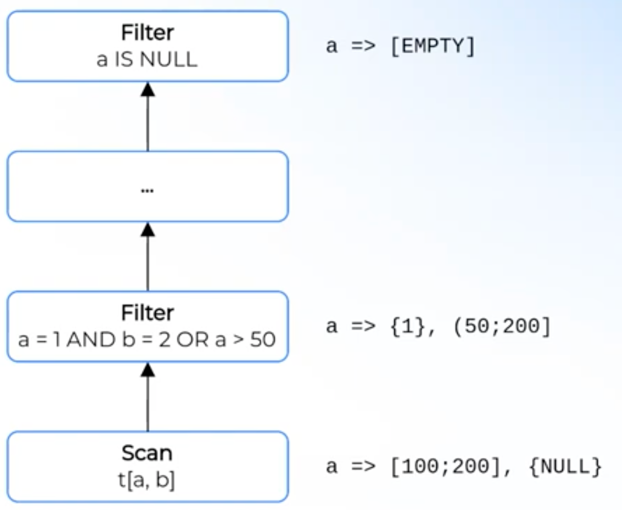
\includegraphics[width=\textwidth]{Pictures/Metadata/Рассчёт ограничений}
        \caption{Пример оптимизации запроса, исходя из ограничений}
        \label{fig:constraints}
    \end{figure}

    \newpage

    \subsection*{Уникальность}

    Исходя из работы операторов можно понять, что некий атрибут уникален, а как следствие упрощение дерево разбора.

    \begin{figure}[h!]
        \centering
        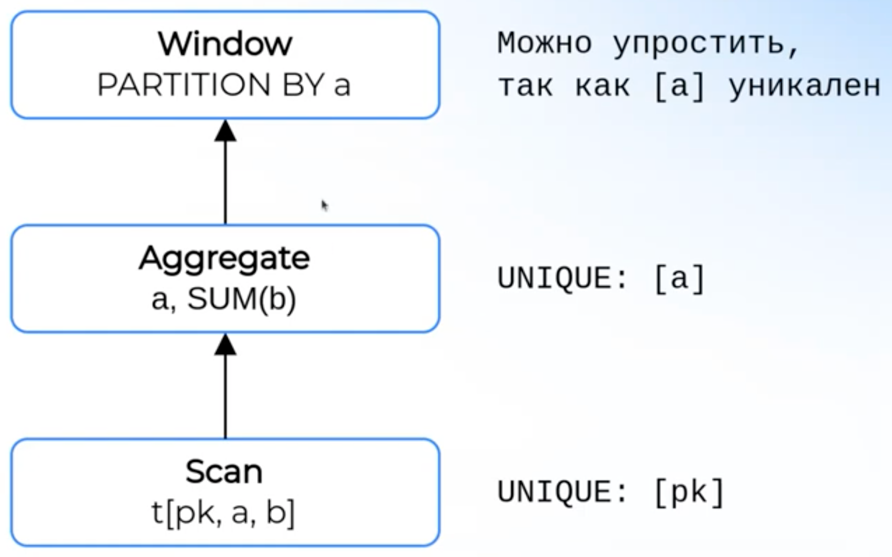
\includegraphics[width=\textwidth]{Pictures/Metadata/Рассчёт уникальности}
        \caption{Пример оптимизации запроса, исходя из уникальности}
        \label{fig:unique}
    \end{figure}

    \newpage

    \subsection*{Свойства}

    \textbf{Свойство} --- характеристика данных, которую можно изменить путём добавления к плану специального оператора к плану.
    Примеры:

    \begin{itemize}
        \item \textbf{Sortedness} - Отсортированность кортежей в отношении.
        Используется, например, в merge sort.
        \item \textbf{Distribution} - Распределение данных по вычислительным элементам.
    \end{itemize}

    \begin{figure}[h!]
        \centering
        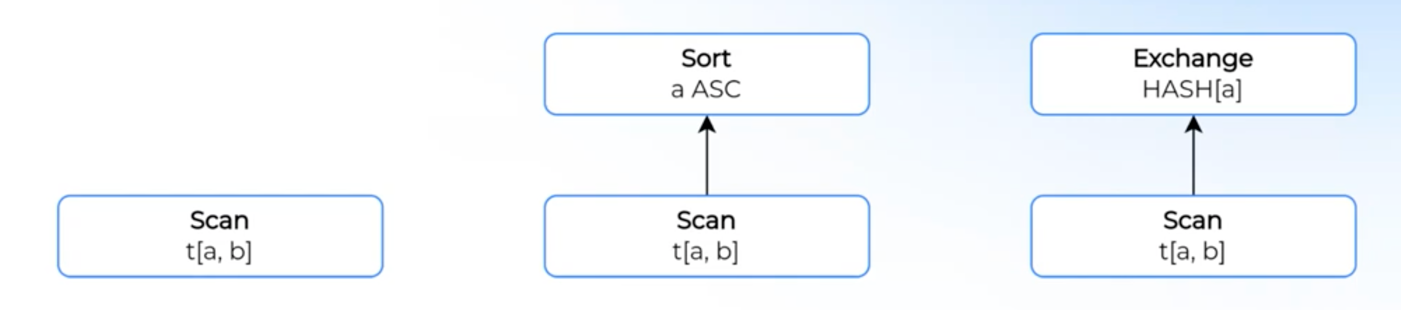
\includegraphics[width=\textwidth]{Pictures/Metadata/Изменение свойств}
        \caption{Пример добавления операторов для изменения свойств}
        \label{fig:properties}
    \end{figure}

    \newpage

    \section*{Оптимизация запросов}
    \newline
    \textbf{Эквивалентные планы} --- планы, производящие эквивалентные отношения для любых входных данных.

    \textbf{Стоймость плана} --- величина, описывающая трудоёмкость его выполнения (Какой-то скаляр/вектор/\ldots)

    \textbf{Трансформация плана} --- замена текущего плана на эквивалентный.
    Производится с целью снижения стоймости плана.

    \textbf{Оптимизация} --- последовательность трансформаций плана.

    \subsection*{Visitor}

    Многие системы используют паттерн \texttt{Visitor}.
    Пример кода указан выше.

    \begin{itemize}
        \item Позволяет обойти узлы плана в заданном порядке.
        \item Позволяет реализовать любую логику.
        \item Крайне громоздкий, поэтому используется для больших и сложных оптимизаций.
    \end{itemize}

    \subsection*{Rule-based оптимизация}

    \begin{lstlisting}[language=Java,
        label={lst:rule}]
        class Rule {
            Pattern getPattern();
            PlanNode apply(Capture context);
        }
    \end{lstlisting}

    \begin{itemize}
        \item Изолированная трансформация, которую оптимизатор применяет к отдельной части плана в соответствии паттерном.
        \item Паттерн - логика сопоставления паттерна с определённым участком кода.
        \item Поиск паттерна может быть осуществлён разными алгоритмами.
    \end{itemize}

    \begin{figure}[h!]
        \centering
        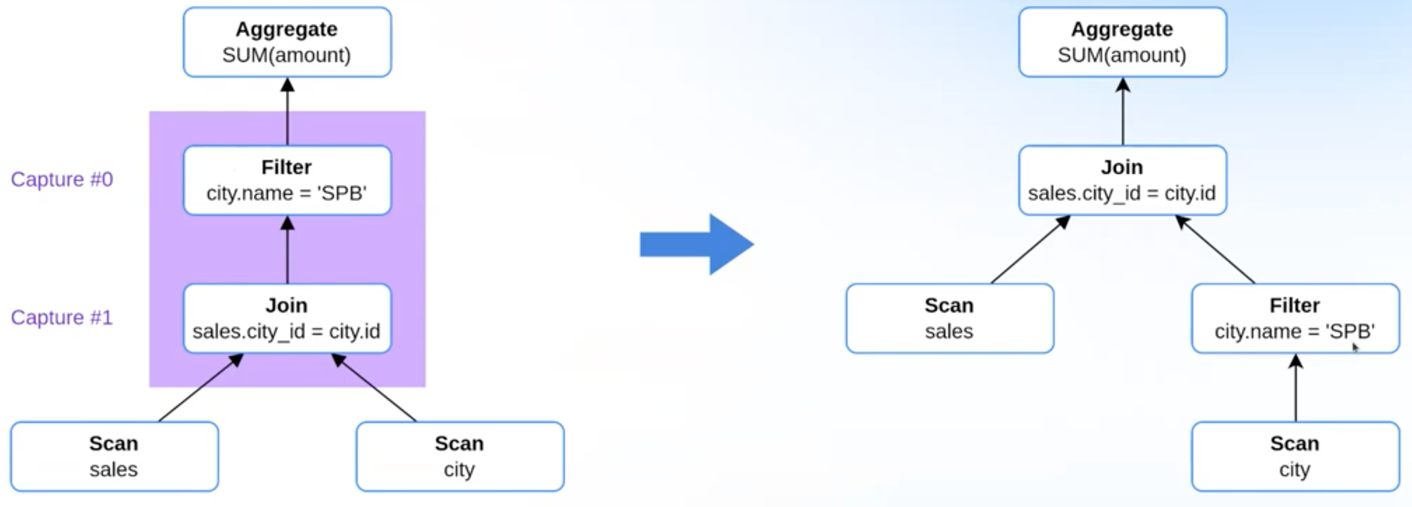
\includegraphics[width=0.7\textwidth]{Pictures/Optimisations/Rule-based}
        \caption{Пример матчинга паттерна и последующей оптимизации}
        \label{fig:figure}
    \end{figure}

    \subsubsection*{Итеративный драйвер}

    Простейший паттерн, который проходит по дереву операторов, метча паттерны и выполняя изменения.

    \begin{itemize}[label=-]
        \item Не учитывает специфику данных, из-за чего применённые оптимизации могут не давать выигрыша
        \item Возможна проблема зацикливания.
        \begin{figure}[h!]
            \centering
            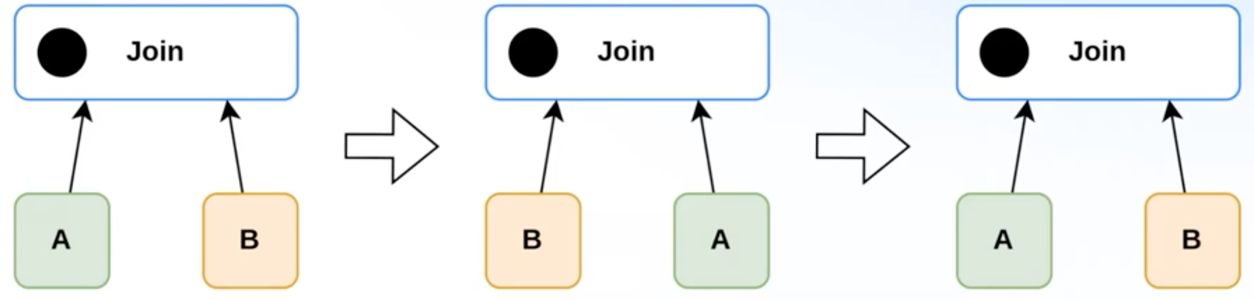
\includegraphics[width=0.6\textwidth]{Pictures/Optimisations/Зацикливание}
            \caption{Пример зацикливания}
            \label{fig:cycle}
        \end{figure}
        \item Может зависеть от порядка обхода и вследствие чего может оказаться недооптимизированно.
    \end{itemize}

    \subsubsection*{Драйвер с мемоизацией}

    \begin{figure}[h!]
        \centering
        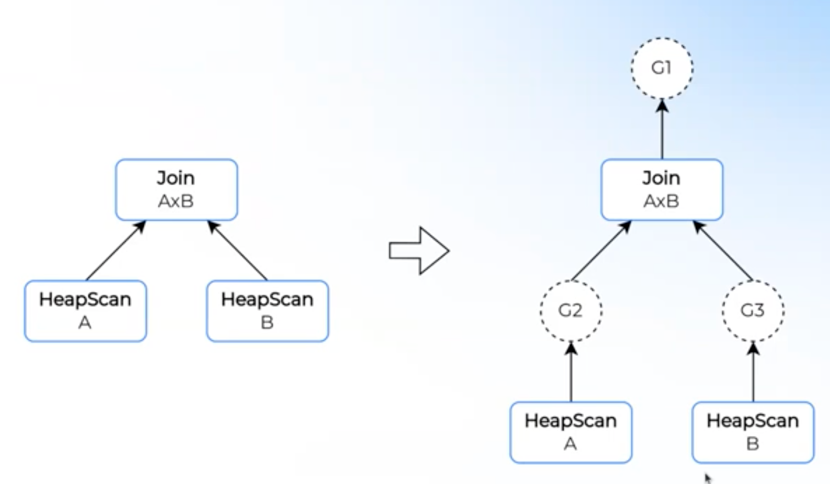
\includegraphics[width=0.6\textwidth]{Pictures/Memo/Граф в Memo}
        \caption{Пример перевода из обычного графа в MEMO}
        \label{fig:graph_to_memo}
    \end{figure}

    \textbf{MEMO} --- структура данных, которая позволяет компактно хранить большое количество планов.
    Представляет собой чередование тех операторов, что у нас были в старых графах и групп эквивалентности, содержащих один или несколько реальных узлов.

    Memo крайне удобно добавление новых узлов, изменение в узле = ещё один AND оператор на входе в OR\@.
    Более того изменения порядка узлов также могут выглядеть не сложно и не опираться на реализацию драйвера.

    Ещё одним плюсом Memo является простота поиска наиболее дешёвого плана.
    Если дать вершинам стоймость, то можно найти оптимальное дерево, выбирая на каждом OR оптимальную вершину.
    
    \begin{figure}[h!]
        \begin{minipage}[t]{\linewidth}
            \centering
            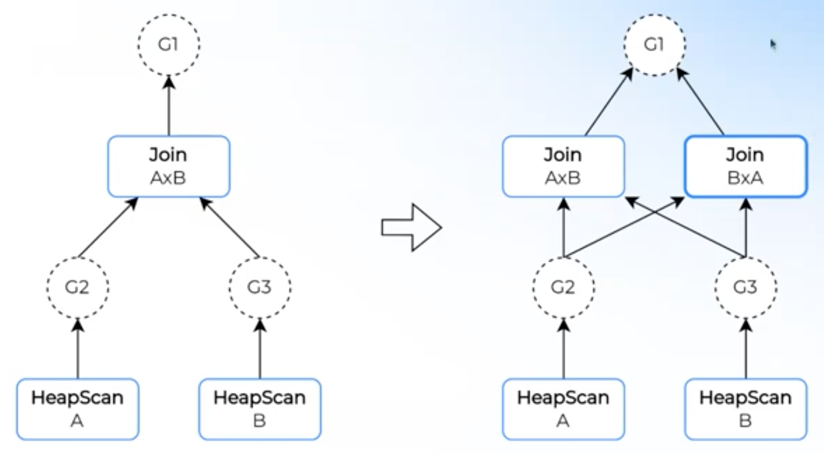
\includegraphics[width=0.6\textwidth]{Pictures/Memo/Добавление узла в Memo}
            \caption{Добавление узла в Memo}
        \end{minipage}
        \begin{minipage}[b]{\linewidth}
            \begin{lstlisting}[language=Java,label={lst:filter_join_transpose},caption={Пример правила перестановки}]
                class FilterJoinTranspose {
                    Pattern pattern = filter().join();

                    void apply(Context context) {
                        Operator filter = context.get(0);
                        Operator join = context.get(1);

                        Operator newJoin = new Join(filter.replace(join.left()), join.right());
                        return newJoin;
                    }
                }
            \end{lstlisting}
        \end{minipage}
        \label{fig:adding_to_memo}
    \end{figure}

    \begin{figure}[h!]
        \centering
        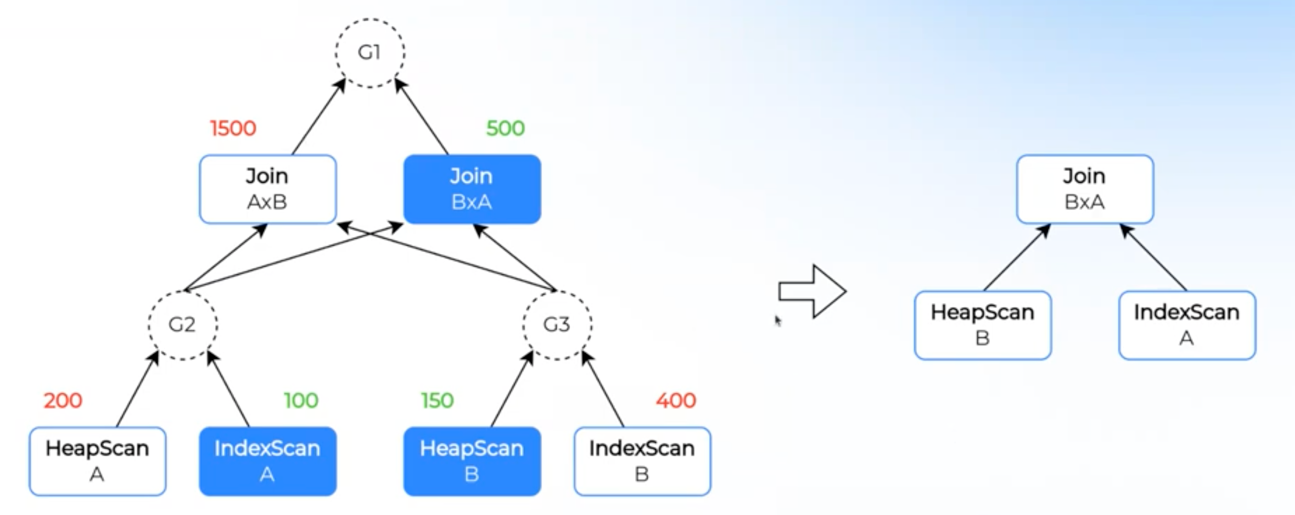
\includegraphics[width=0.6\textwidth]{Pictures/Memo/Стоймость в Memo}
        \caption{Выбор оптимального дерева.}
        \label{fig:cost_in_memo}
    \end{figure}

    \newpage

    \subsubsection*{Properties and enforcers}

    Некоторые операторы задают требования к свойствам своего входа, поэтому можно либо добавить узлы, чтобы операторы имели такие свойства (например отсортировать) или проверить, что оно выполняется.

    \begin{figure}[h!]
        \centering
        \includegraphics[width=0.6\textwidth]{Pictures/Memo/Properties и enforcers}
        \caption{Оптимизация по properties}
        \label{fig:properties_enforcers}
    \end{figure}
    
    \newpage
    
    \subsubsection{Cascades}
    
    \textbf{Cascades} - алгоритм, который использует MEMO, rule-based оптимизацию и управление свойствами для поиска оптимальных планов.
    Мы можем совмещать оптимизации, спускаясь и поднимаясь по операторам и изменяя, если это принесёт оптимизацию.

    \begin{figure}[h!]
        \centering
        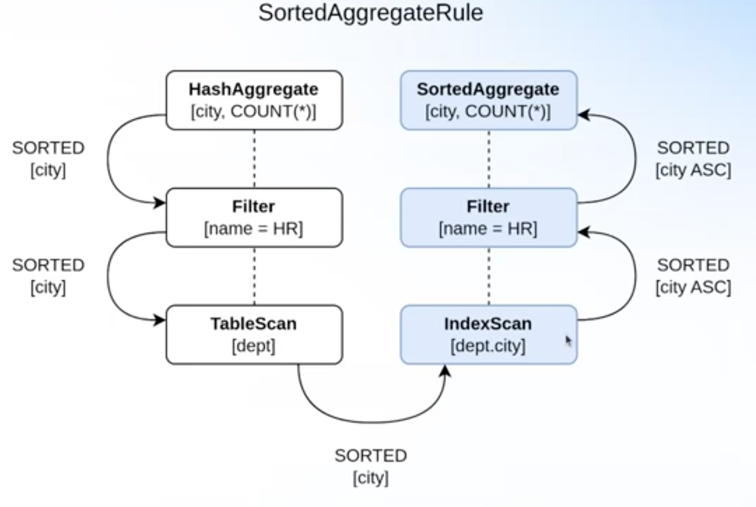
\includegraphics[width=0.6\textwidth]{Pictures/Cascades}
        \caption{Спуск в Cascades до TableScan}
        \label{fig:cascades}
    \end{figure}

    Однако такая технология может быть не во всех базах данных, так как несмотря на плюсы, сам алгоритм достаточно сложный и может привести к неожиданным эффектам.

    \subsection*{Итоги}

    Оптимизаторы зачастую используют комбинации алгоритмов.
    Так они могут использовать iterative, потом cascades\ldots
    Делается это чтобы количество планов не разрасталось из-за больших оптимизаторов.
\end{document}
